\documentclass[11pt]{article}
\usepackage[a4paper, margin=2.7cm]{geometry}
\clubpenalty=10000 \widowpenalty=10000
\usepackage{graphicx}
\usepackage{booktabs}
\usepackage{amsmath}
\usepackage[hidelinks]{hyperref}
\hypersetup{pdftitle={StillDrawn: Measuring the Stability of Inked Line Art under Image-to-Video Generation},pdfauthor={Aaron Smiles}}
\usepackage{xcolor}
\newcommand{\todo}[1]{\textcolor{red!70!black}{[TODO: #1]}}
\newcommand{\datadoi}{\href{https://doi.org/10.5281/zenodo.23072784}{10.5281/zenodo.23072784}}
\newcommand{\coderepo}{\url{https://github.com/aaronlsmiles/stilldrawn}}

\title{StillDrawn: Measuring the Stability of Inked Line Art\\
under Image-to-Video Generation}
\author{Aaron Smiles\\ \small Independent researcher, UK}
\date{}

\makeatletter
\def\bstctlcite{\@ifnextchar[{\@bstctlcite}{\@bstctlcite[@auxout]}}
\def\@bstctlcite[#1]#2{\@bsphack
  \@for\@citeb:=#2\do{%
    \edef\@citeb{\expandafter\@firstofone\@citeb}%
    \if@filesw\immediate\write\csname #1\endcsname{\string\citation{\@citeb}}\fi}%
  \@esphack}
\makeatother
\begin{document}
\maketitle
\bstctlcite{IEEEexample:BSTcontrol}

\begin{abstract}
Inked line art is an unforgiving substrate for image-to-video generation:
line weight, screentone frequency, contour closure and the black-and-white
register itself must survive every frame. We introduce \textbf{StillDrawn},
a benchmark for that survival: a 29-panel dataset controlled for content
class and ink treatment, five frozen-definition stability metrics,
and a pre-registered study of 171 protocol cells on five engines (two
open-weights models from pinned quantisations, three hosted commercial
systems) yielding 170 clips and one recorded refusal. The pre-registered
hypothesis, that establishing-shot panels degrade more than character and
action panels, returned null on all ten engine--metric tests; reported as
registered. Instead, the corpus shows a seven-mode failure taxonomy on three
axes (register, content, framing): modes that stay monochrome ink to the eye
while the metrics read catastrophe (in-register \emph{transposition}) and
modes the metrics barely see (in-register \emph{insertion}: a hallucinated
cyclist at $0.47$\,px mean line drift, the corpus's tenth percentile). A
pre-registered human check (six raters, two axes, per-panel baseline)
validates the suite on the axis that can be anchored: four of five metrics
track perceived content preservation (edge $\rho = -0.74$,
$p = 2\times10^{-4}$; Krippendorff's $\alpha = 0.48$), while the absolute
ink-register judgement is bounded by the corpus: raters concur that the
source panels behind nearly a third of the clips do not read as hand-drawn.
A caution generalises beyond line art: a post-hoc optical-flow control shows
our engine ordering tracks how much each engine \emph{moves} ($\rho = 0.90$,
median motion vs median line drift), with no motion regime where all five
engines are comparable; stability scores on any substrate rank stillness
unless a motion control is reported with them. Dataset, recipes, metrics and
all 373 generated clips are released.
\end{abstract}

\section{Introduction}

\begin{figure}[t]
\centering
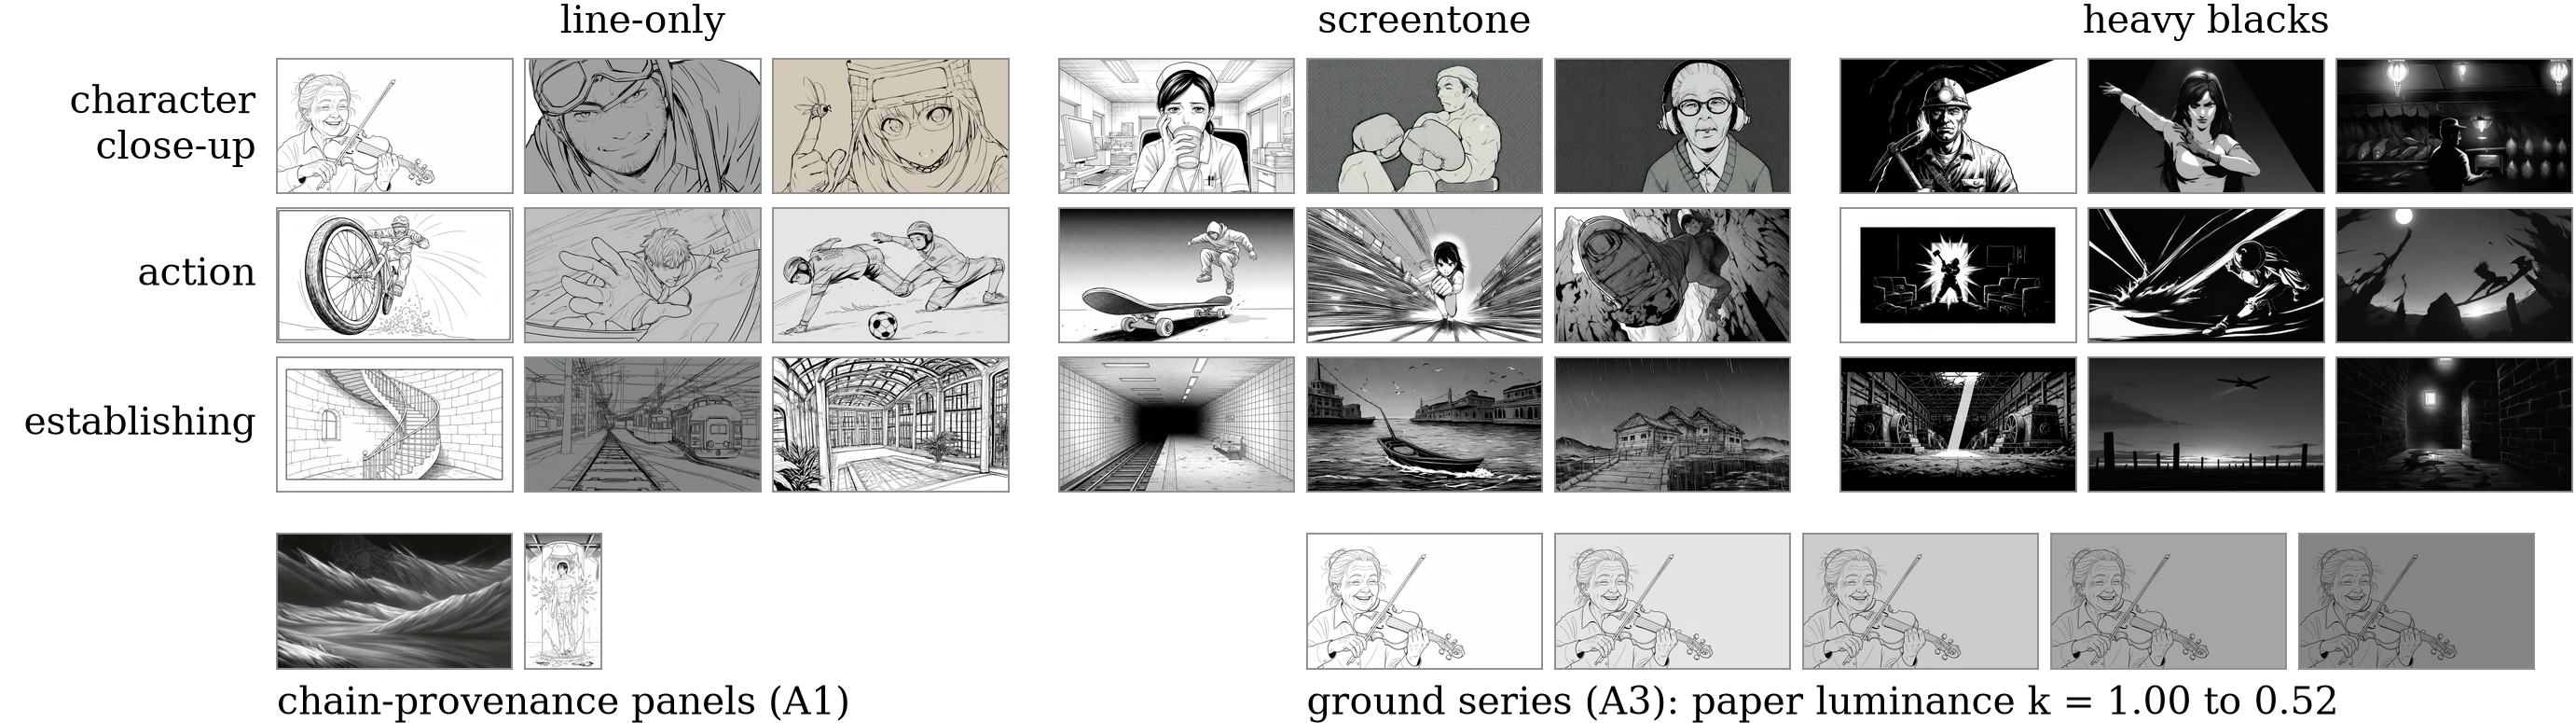
\includegraphics[width=\linewidth]{../analysis/out/figures/panel_grid.png}
\caption{The StillDrawn panels. Top: the 27 core panels of the
$3\times3\times3$ design, one row per content class and three columns per ink
treatment. Bottom left: the two chain-provenance panels, a cosmic
establishing panel and the creator-IP action panel (native portrait). Bottom
right: the five ground variants of one line-only panel used in
Section~\ref{sec:ground}, with luminance scaled globally by $k = 1.00$ to
$0.52$, which greys the paper. Every panel is released with its line-art layer and recipe.}
\label{fig:panels}
\end{figure}

Comics and manga production is converging on a hybrid practice in which
generative models propose and a human artist disposes. For moving panels (animatics, motion comics, ``living'' establishing shots),
the proposing model is an image-to-video (I2V) system conditioned on a finished, inked panel. The
craft question is narrow and unforgiving: \emph{does the clip remain a drawn
black-and-white ink image, frame by frame?} A panel that drifts into
photographic rendering, grows tonal shading its style never had, or letters
itself with pseudo-text has not animated the drawing; it has replaced it.

This work is motivated by a studio practice we call
\emph{sample-then-commit}: the artist generates a rough cloud of candidate
strokes or plates, consolidates, and only then commits ink. The
consolidation step is where authorial control lives. Two things about that
practice shape this paper: first, that intuitions about what generative
processes preserve are cheap and
often wrong (our own registered hypothesis, reported below, is an
instance), so evaluation must be pre-registered; second, that the
stability of the \emph{inked register itself} under generative transformation
is the load-bearing assumption of any such practice, universally assumed
and measured only obliquely. Where it is measured at all, it is measured as
compliance with a control signal the generator was handed, or as a human
judgement internal to one model's own development
loop~\cite{huang2024lvcd,tencent2026animatrix}. What is missing is a measure
of whether the register survives when nothing is holding it in place.
StillDrawn supplies that. The failure itself is not unknown to practitioners:
a case study of AI-assisted manga production notes in passing that a driven
monochrome panel acquired ``photorealistic features like lips and
teeth''~\cite{zhang2025panelsouls}. That is a single qualitative observation
in a limitations paragraph: the mode is
recognised anecdotally and has not been measured.

Two observations from the surrounding literature shape what follows. First,
the rough-sketch cleanup benchmark of Yan et al.~\cite{yan2020cleanup}, which
defines the register we measure, names as future
work precisely the evaluation we undertake: ``end-to-end evaluations on
specific downstream sketch processing tasks like 3D reconstruction \dots\ or
animation in-betweening''. Second, in the closest standardisation study for
conditional image generation, ImagenHub~\cite{ku2023imagenhub}
reports that across roughly thirty models and seven tasks, no existing
automatic metric reaches a Spearman correlation of $0.2$ with human
judgement outside a single task. The same gap has been shown on drawn
content specifically: the AniSora authors abandoned general-purpose scores
for animation after finding that a clip with visible distortions outscored a
clean one on motion smoothness~\cite{jiang2024anisora}. A metric suite for a
new substrate therefore cannot be validated by construction; it has to be
checked against people, which is why Section~\ref{sec:human} exists and why
we registered its predictions before rating began.

\paragraph{Contributions.}
(1)~A 29-panel dataset controlled for content class (character close-up /
action-foreshortened / establishing environment) and ink treatment
(line-only / screentone / heavy-blacks), each panel with its extracted
line-art layer, generation recipe (full for 27 panels, described for the two
chain-provenance panels of Section~\ref{sec:dataset}), and measured ground
covariates;
(2)~five automatic stability metrics with definitions frozen before any
benchmark generation, validated on pilot clips, and released as a single
self-documenting tool;
(3)~a pre-registered, budget-disclosed cross-engine study (five engines, 171
cells), whose registered hypothesis test returned null and is reported as
such;
(4)~a failure-mode taxonomy: seven named modes on three axes, each with
$\geq 2$ independent exemplars and a stated metric signature, including two
systematic blindness directions of global metrics;
(5)~a pre-registered human check (six raters, two axes, per-panel
baseline) that validates four of five metrics against perceived content
preservation (the \emph{sameness} axis), quantifies the metric--perception divergence on the insertion mode (the
only pre-stated per-mode prediction the seeded subset could test; its
transposition coverage gap is reported, not repaired), and shows the
absolute register judgement to be bounded by the corpus itself (source panels
naive raters do not read as hand-drawn) rather than by engine behaviour. Rater materials and the hosted instrument are
released.

\section{Related work}
\label{sec:related}

\textbf{Stroke consolidation and sketch cleanup.} A mature line of work
treats line drawings as first-class geometry: trainable stroke clustering
and curve fitting, crowdsourced drawing correction, learned sketch
simplification and inking, aggregation of vector strokes, and
perception-driven
consolidation~\cite{orbay2011beautification,limpaecher2013crowd,%
simoserra2016simplify,simoserra2018mastering,simoserra2018inker,%
liu2018strokeaggregator,pagurek2021strokestrip,liu2023stripmaker,%
yan2024vectorization,yu2024sketchbeaut}, with a dedicated benchmark for
rough-sketch cleanup~\cite{yan2020cleanup}. This literature defines the
\emph{register} whose survival we measure (closed contours, deliberate
line weight, screentone as a frequency structure) but evaluates static
consolidation, not temporal stability.

Two conventions of that literature carry directly into our design. It scores
geometric agreement between drawings with the symmetric chamfer distance:
Yan et al.~\cite{yan2020cleanup} adopt it after comparing alternatives, and the
recent part-level beautification work of Yu et
al.~\cite{yu2024sketchbeaut} reports mean chamfer distance, beside Earth
Mover's Distance, as its quantitative faithfulness measure. That is why \texttt{line\_drift} reduces to a
chamfer headline (Section~\ref{sec:metrics}). And it pairs that geometry with
a perceptual study rather than trusting it alone, on the grounds that the
judgement being modelled is ultimately a human one. Our Section~\ref{sec:human}
follows the same two-part pattern, with the difference that we register its
predictions in advance.

One boundary on that convention is worth stating, because it is the sharpest
available objection to a chamfer headline. Yan et al.\ also ran a pilot
correlating cleanup metrics against human ratings, and chamfer's agreement
with raters differed markedly between their two test drawings ($r=-0.87$ and
$r=-0.33$). The confound they identify is line thickness: one compared method
emitted systematically thicker strokes, and excluding it moved both
correlations up ($-0.90$ and $-0.56$), making chamfer the most highly
correlated metric on both drawings. Two things
follow for us. That pilot is small (two drawings, twelve stimuli per
correlation, naive raters) and its authors attribute the inconsistency to the
study rather than the measure. And its confound does not arise here: StillDrawn
holds one inked substrate fixed rather than comparing nine methods whose
stroke weights could not all be equalised. We are nonetheless explicit about what \texttt{line\_drift}
does and does not claim: it measures \emph{line displacement}, not perceived
\emph{quality}, and Section~\ref{sec:human} tests the relationship between the
two rather than assuming it.

That distance-transform convention has already been carried into generated
video. Line-art video colourisation is evaluated with a sketch-alignment
measure that extracts line maps from generated frames and scores their
displacement against a reference drawing via a Euclidean distance
map~\cite{huang2024lvcd}, a construction reused in later animation
work~\cite{li2026sketchkeyanime}. \texttt{line\_drift} is the same family of instrument, and we claim no
novelty for the mechanism. The difference is what the reference is and what
the number therefore means: those measures score \emph{compliance}, asking
whether output frames obey a per-frame sketch supplied as a control signal,
so a low score indicates a controller working as designed. Ours scores
\emph{drift} in the absence of any such control (displacement from the
source panel and from frame zero under a free-running I2V model), where
there is nothing holding the geometry in place and no per-frame target to
comply with.

\textbf{I2V generation and its evaluation.} Video generation is typically
scored distributionally (the Fr\'echet Video Distance, FVD, and its family), by text alignment, or by general
video-quality suites~\cite{huang2023vbench,liu2023evalcrafter}; none of these
is a per-clip measure of whether a drawn
substrate remains drawn. Closest in spirit are works on animating line art
and manga
directly~\cite{meng2024anidoc,zhang2025panelsouls,zhan2025coprosketch},
which report style preservation qualitatively; and diffusion-prior
repurposing work~\cite{ke2023marigold,thawatdamrongkit2026dma} for the
pattern of extracting a controlled signal from a generative prior. StillDrawn differs in evaluating
\emph{engines as products} on a fixed dataset with released recipes and frozen
per-clip metrics.

Animation-specific evaluation has a short but real history.
AniSora~\cite{jiang2024anisora} assembles 948 animation videos with
animation-tuned metrics for character and art-style consistency, motivated by
the observation that general-purpose scores diverge from human judgement on
animated content; AnimationBench~\cite{wu2026animationbench} benchmarks
animation I2V across nineteen dimensions grounded in the twelve basic
principles of animation and in IP preservation, scored largely by
vision--language judges. Both work in colour, character-centric
animation: neither treats screentone or the black-and-white register, and no
dimension in either asks whether a drawn substrate is still drawn. They are
therefore complementary to this work: they measure whether an animated
character acts well and looks like itself; we measure whether the ink
survives.

Two recent results indicate the constructs we measure are the right ones. A
production anime generation system~\cite{tencent2026animatrix} reports, among
scores assigned by professional evaluators, a diagnostic \emph{Line-Art
Quality} subscore defined over ``outline continuity, edge crispness, and line
flicker'', independently arriving at close variants of our closure,
\texttt{edge\_decay} and \texttt{line\_drift} channels. That subscore is a
human 1--5 judgement used to compare two versions of one model; StillDrawn
supplies frozen automatic equivalents, defined in advance and comparable
across engines. One
contrast is worth drawing out, because the same measurement carries opposite
meaning in the two designs: AnimationBench samples five videos per input to
score \emph{Diversity}, treating variation across draws as a desirable
property, whereas Section~\ref{sec:repeat} treats that variation as the thing
that determines what a single benchmark score can mean.

\textbf{Failure taxonomies for generated video.} Categorising generative
failure is established practice.
BrokenVideos~\cite{lin2025brokenvideos} annotates 3{,}254
generated videos with pixel-level artefact masks under a five-category
taxonomy (technical, semantic, cognitive, consistency, instructional), in
which \emph{style inconsistency} covers transitions such as realism turning
to cartoon; Artifact-Bench~\cite{tang2026artifactbench} extends this to a
three-level hierarchy spanning photorealistic, animated, and CG-style video;
and hallucination taxonomies for video--language models make a parallel
division~\cite{huang2026distorted}. Our taxonomy differs from these in its
criterion rather than merely its domain, and the distinction is worth being
precise about, because Artifact-Bench does cover stylised content. Those
taxonomies organise failure around \emph{realism}: their tasks are
real-versus-generated classification, pairwise realism comparison and
fine-grained artefact identification, and an
artefact is a departure from physical or perceptual plausibility. Ours
organises failure around \emph{drawnness}. The two criteria are not merely
different but in places opposed: our A3 register collapse, in which an
inked panel resolves into photographically lit rendering, is a total failure
under our criterion and would count as an improvement under theirs. Our
modes are also each paired with a measured metric signature, including two
directions in which global scalars are systematically blind, rather than
being built to train localisation models (Section~\ref{sec:taxonomy}).

\textbf{Reliability under repeated inference.} Our repeat analysis
(Section~\ref{sec:repeat}) imports a framing developed in large language model (LLM) safety
evaluation rather than inventing one. Accelerated Prompt Stress
Testing~\cite{broadwater2026apst,broadwater2026reliability}
distinguishes \emph{breadth-oriented} benchmarks from \emph{depth-oriented}
evaluation that repeatedly samples identical prompts, and models the
resulting failures as Bernoulli outcomes with per-inference failure
probabilities rather than as isolated events. That work is
text-only. We are not aware of an equivalent treatment in image-to-video
generation: the recent survey of AI-generated video
evaluation~\cite{liu2024survey} does not raise generation stochasticity or
repeat sampling as an evaluation problem.

\textbf{Perceptual grounding and reporting practice.} Our human-check design
follows ensemble-perception findings that observers form reliable summary
judgements over brief exposures~\cite{ariely2001sets,whitney2018ensemble},
and adopts the rater protocol of
ImagenHub~\cite{ku2023imagenhub}, which standardises
human evaluation of conditional image generation with three raters per model
and Krippendorff's $\alpha$ as the reliability statistic. Our
dataset documentation follows Gebru et al.~\cite{gebru2021datasheets}; and
the frozen-protocol-with-dated-amendments reporting practice is borrowed
from pre-registration norms in the experimental
sciences~\cite{nosek2018preregistration}, which have
been argued for in machine learning~\cite{bell2021perspectives,leech2024questionable} but are, to
our knowledge, not yet applied to cross-engine generative-video evaluation.

\section{Dataset}
\label{sec:dataset}

\textbf{Core.} Twenty-seven neutral panels form a $3\times3\times3$ design
(Figure~\ref{fig:panels}):
three content classes (character close-up \texttt{cu}, action-foreshortened
\texttt{act}, establishing environment \texttt{est}) $\times$ three ink
treatments (line-only, screentone, heavy-blacks with one reserved white
region) $\times$ three panels per cell, all at $1344\times768$. Subjects are
original and neutral (a violinist, a boxer, a lighthouse interior; no named
properties, no real people, no text). Panels were generated through a
recorded harness (nine via a hosted prose-prompt engine, eighteen via a
local tag-prompt engine), deliberately mixing generators so the dataset is
not single-engine-biased. Every panel ships with a machine-readable recipe
(engine, model, prompt, negative, seed, settings, date, reroll flag), a
line-art layer extracted with the same weights used by the metric suite, and
measured covariates.

\textbf{Chain-provenance additions.} Two further panels entered the matrix before any
benchmark generation, their cells assigned by dated amendment (A1; the
creator-IP panel itself was admitted under the frozen protocol's optional
creator-IP clause): a creator-IP action panel
from the author's comic project (cleared panel-by-panel; two sibling
candidates were refused and are absent), and a neutral cosmic establishing
panel built through the same private production chain. Both carry
\emph{described-not-reproducible} recipes: the chain is named (line
extraction $\to$ inversion $\to$ img2img inking), its tunings withheld;
the benchmark ships evaluation artefacts, not the production stack.

\textbf{Covariates instead of rerolls.} Local line-only generation often
renders the paper ground light grey rather than white. After one recorded
reroll round we kept the grey-ground panels as authentic engine output and
recorded per-panel \emph{paper-white p90} (90th-percentile) luminance and black-pixel fraction
in the datasheet. Section~\ref{sec:ground} shows this covariate earning its
place. A datasheet in the Gebru et al.~\cite{gebru2021datasheets} structure
documents composition, provenance, known marks (including SynthID on the
hosted panels), deviations, and limitations.

\section{Metric suite}
\label{sec:metrics}

Five per-clip metrics, each reducing to one frozen headline scalar; all
frames are analysed at native clip resolution, and every result JSON embeds
the normative definitions verbatim.

\begin{enumerate}
\item \textbf{line\_drift}: per-frame line maps from the same
  anime-line-art extractor used for the dataset layers, binarised at a per-map
  Otsu threshold; symmetric chamfer distance and tolerance-IoU of frame~$t$ vs
  frame~0 and vs the source layer. Headline: mean chamfer vs frame~0 (px).
\item \textbf{tone\_spectral\_drift}: Hann-windowed 2-D FFT over 64\,px
  tiles inside a tone mask (local-mean mid-grey of the source panel; halftone
  pixels are bimodal, only their local average is grey); the frame-0
  dominant radial bin fixes a band; headline: variance of the per-frame
  band-energy fraction. Undefined (and reported as such, never imputed) on
  panels with fewer than four qualifying tiles.
\item \textbf{edge\_decay}: Sobel gradient-magnitude 95th percentile per
  frame; headline: \emph{magnitude} of the normalised slope. The magnitude
  headline was fixed during pilot validation, before the freeze: photoreal
  drift can \emph{raise} edge energy (added photographic texture) as well as
  lower it (softening); the signed slope is reported alongside and its sign
  feeds the taxonomy.
\item \textbf{style\_drift}: DINOv2 ViT-S/14 CLS-embedding cosine
  distance of frame~$t$ vs frame~0; headline: terminal distance. (Checkpoint
  checksum recorded in the release.)
\item \textbf{closure\_proxy}: density of skeleton endpoints in the
  binarised line maps; headline: $|$terminal drift$|$ vs frame~0.
\end{enumerate}

Validation on three pre-benchmark pilot clips required the suite to
reproduce a known perceptual ranking (an establishing shot that visibly
dissolved towards photo-rendering had to rank worst on style and edge); it
did, after the edge-decay sign lesson above, and the definitions were then
frozen.

\section{Pre-registered protocol}
\label{sec:protocol}

The full protocol (metric definitions, motion prompts, run matrix, human
check, taxonomy seeding rule, and analysis plan) was frozen in a
pre-registration document before any benchmark batch ran and committed to
version control. It changed afterwards only through dated amendments, A1--A8 (nine in all:
the label A6 was used twice, for the motion channel of 2026-08-14 and the
human-check instrument of 2026-08-15, as the release's provenance record
notes, and we cite each by topic; the first two admit the chain-provenance panels and move the open-weights
engines to a rented CUDA GPU with identical pinned weights, quantisations,
seeds, and settings); all are released with the document. The development
history itself is private; the release lists the freeze and amendment
commits by hash and date.

\textbf{Run matrix.} Five engines: Runway Gen-4 Turbo and Gen-4.5 (hosted),
MiniMax H3 via fal.ai (hosted), Wan~2.2 TI2V-5B and LTX-2.3-22B-distilled
(open weights, pinned GGUF quantisations; hereafter Turbo, Gen-4.5, H3, Wan
and LTX). Per engine, 33 cells: each of the 27 core panels
once, with motion class assigned by a fixed rotation over
IDLE / BURST / CAMPUSH, and the two chain-provenance panels under all three
classes (amendment A1); five seconds; motion prompts frozen verbatim, with an
identical style-lock sentence in each of the three classes; plus six first$\to$last interpolation cells
(FLINT) on the one engine that supports first$\to$last conditioning,
MiniMax H3. Model
identifiers, version strings, dates, resolutions, and costs are pinned per
clip in the released manifest; execution hardware is recorded per batch
(Table~\ref{tab:engines}). Moderation and API
failures follow a frozen rule: one identical resubmission, then the cell is
recorded as refused: a result, not a gap. The frozen run matrix ran
inside a disclosed \pounds50 budget ceiling (\pounds43.53 spent). Each
extension that followed was logged in the ledger before the next batch was
submitted: the repeat-stability probe of Section~\ref{sec:repeat}, the ground
series of Section~\ref{sec:ground}, and two registered amendments not analysed
further in this paper, a hazard-rate study and a second-engine scout
(amendments A4 and A5, whose clips, scores and registered analyses are
released). In A4, ten MiniMax H3 draws per cell on eight cells gave per-cell
departure rates from 0\% to 90\%, and the registered one-sided Fisher test
(BURST$\times$heavy-black 12/20 against IDLE$\times$line-only 9/20) was null,
$p = 0.26$; the A5 scout stopped at its registered three-draw look, one draw of
three departing under the frozen rule, and is reported as a pilot with no rate
claim. The extensions brought total spend to \pounds115.37; the ceilings were
retired on 2026-08-14 in favour of a per-batch variance rule. Every hosted and every rented-GPU batch is in the
released ledger; the one batch without a row is the five \pounds0 LTX-2.3
ground clips of Section~\ref{sec:ground}, run locally.

\begin{table}[h]
\centering\footnotesize\setlength{\tabcolsep}{4pt}
\begin{tabular}{@{}llll@{}}
\toprule
Engine & Pinned version (manifest, per clip) & Grid & Run date \\
\midrule
Gen-4 Turbo & Runway dev API, X-Runway-Version 2024-11-06 & $1280\times720$ & 2026-08-12 \\
Gen-4.5 & Runway dev API, X-Runway-Version 2024-11-06 & $1280\times720$ & 2026-08-12 \\
MiniMax H3 & fal.ai \texttt{minimax/h3/image-to-video}, 768P & $1344\times768$ & 2026-08-12 \\
Wan~2.2 TI2V-5B & GGUF Q5\_K\_M, ComfyUI 0.31.0, RTX 5090 & $1280\times704$ & 2026-08-12 \\
LTX-2.3-22B & distilled-1.1 GGUF Q4\_K\_M, ComfyUI 0.31.0, RTX 5090 & $1280\times704$ & 2026-08-12 \\
\bottomrule
\end{tabular}
\caption{Engine versions as pinned per clip in the released manifest
(portrait tank cells swap each grid's orientation). Full version strings
(incl.\ text encoders and VAEs), seeds where settable (the open-weights
engines; null for the hosted ones), wall-clock, and per-clip cost are in
\texttt{runs/manifest.jsonl} (the five Wan~2.2 ground clips are listed in
\texttt{runs/manifest-supplement.jsonl}). Hardware is per batch: the open-weights run
matrix ran on a rented RTX 5090; of the ground series
(Section~\ref{sec:ground}), the five LTX-2.3 clips ran on the author's
Apple-silicon machine (MPS backend; their manifest lines carry no hardware bracket,
so this caption is their record) and the five Wan~2.2 clips on a rented RTX
A6000.}
\label{tab:engines}
\end{table}

\section{Results}
\label{sec:results}

All numbers derive from the released per-cell table; the analysis scripts
regenerate every table and figure from the metric JSONs.

\subsection{Engine league and the motion confound}
\label{sec:league}

On median headline scalars across the 33 standard cells per engine, the
open-weights Wan~2.2 is the most stable engine on four of five headlines
(line, tone, style, closure), with Gen-4 Turbo taking the fifth (edge
$|$slope$|$) and placing second on the other four; Gen-4.5 is fourth or fifth
on every headline except closure (third), and MiniMax H3 is last or
near-last on every headline.

\textbf{That ordering is substantially a ranking of stillness, and we can now
say so quantitatively.} Every metric in the suite is optimised by a clip that
does not move, so a stability score alone cannot separate an engine that holds
the register from an engine that ignores its motion prompt. We therefore added
a post-hoc motion channel (optical flow between consecutive sampled frames,
every second frame, scored
by the mean of the largest 5\% of per-pixel magnitudes, following VBench's
Dynamic Degree control~\cite{huang2023vbench}) and re-analysed all 373
clips. It is not a sixth metric: it was written after the corpus was complete,
is registered as exploratory (amendment A6, motion, 2026-08-14), and is used here only to condition
a frozen result, never to restate one. The prediction that the league would
prove confounded was recorded in the amendment before the engine-level
analysis was run.

It is confounded. Across the five engines, median motion and median line drift
rank together at Spearman $\rho = +0.90$ ($n = 5$ engines; exact two-sided
$p = 0.083$), and the two orderings are identical apart from the final pair
exchanging places (Table~\ref{tab:motion}).

\begin{table}[h]
\centering
\small
\begin{tabular}{lrr}
\toprule
Engine & Motion (norm.\ median; post-hoc) & Line drift (px) \\
\midrule
Wan~2.2      & 0.00080 & 0.780 \\
Gen-4 Turbo  & 0.00194 & 2.642 \\
LTX-2.3      & 0.00248 & 2.798 \\
Gen-4.5      & 0.00734 & 4.788 \\
MiniMax H3   & 0.00396 & 5.384 \\
\bottomrule
\end{tabular}
\caption{Per-engine medians over each engine's standard cells (FLINT
excluded) of the post-hoc motion channel (normalised median optical flow;
exploratory, amendment A6, motion, 2026-08-14) and of line drift (mean
chamfer vs frame~0, px), ordered by line drift. Motion is not a frozen
metric; it conditions the league and restates nothing.}
\label{tab:motion}
\end{table}

Wan~2.2, the engine that leads on four of five headlines, moves the least by a
wide margin: $2.4\times$ less than the next engine and $9\times$ less than
Gen-4.5. Within engines the same association holds on four of the five
(line-drift $\rho$ between $+0.38$ and $+0.58$); Wan is the exception at
$\rho = -0.007$, and for the same reason: it is so uniformly static that
there is almost no motion variance within it for the association to act on.
Pooled over all 164 standard cells, motion predicts every headline
(line $+0.590$, style $+0.446$, tone $+0.432$, edge $+0.372$, closure
$+0.158$).

The league is not \emph{purely} a stillness ranking. Conditioning the
engine--metric association on motion leaves it intact but a third to two-fifths
smaller (line drift $+0.495 \rightarrow +0.297$; style $+0.461 \rightarrow
+0.313$), so engine identity still carries signal. But a substantial part of this
ordering measures how much each engine moves, and
we could not repair it by matching: the five engines' motion interquartile
ranges have no common overlap, so there is no regime in which all five can be
compared at equal movement. In that sense they are not attempting the same task. We
therefore report the league as descriptive, always beside its motion medians,
and not as a quality ranking.

\paragraph{What a motion-controlled comparison does and does not recover.}
Three analyses of the existing corpus test how much of the ordering survives
(Figure~\ref{fig:motion}). \emph{Pairwise matching} restricts each two-engine
comparison to the overlap of their motion interquartile ranges, assuming
nothing about functional form; five of the ten pairs yield a usable band, and
\textbf{two of those five reverse}. MiniMax H3, last on line drift in
Table~\ref{tab:motion}, beats Gen-4 Turbo when the comparison is held at
equal movement (2.46 vs 2.88\,px), and LTX overtakes Turbo (1.83 vs
2.88\,px). Wan~2.2 has \emph{no} usable overlap with any other engine (with
Turbo and H3 the overlap is too thin to use): the engine that leads the
league cannot be compared with any of the field at equal motion from this
corpus at all.
\emph{Model-based matching} (fitting drift on motion per engine and
comparing fitted values at a common motion level) instead preserves the raw
ordering exactly. The two disagree, and that disagreement is the substantive
result: the ranking is not robust to how motion is controlled, so no ordering
derived here should be read as a quality verdict.

What survives is weaker and better founded: a \emph{dominance} statement. An
engine is beaten outright only if another both moves more and drifts less. On
that criterion only H3 is dominated (by Gen-4.5); the remaining four sit on a
frontier along which stability is traded against movement and cannot be
ordered without declaring an exchange rate between them, and that rate is a claim
about what a user wants, not about what an engine does. We report the frontier
and decline to set the exchange rate.

\begin{figure}[t]
\centering
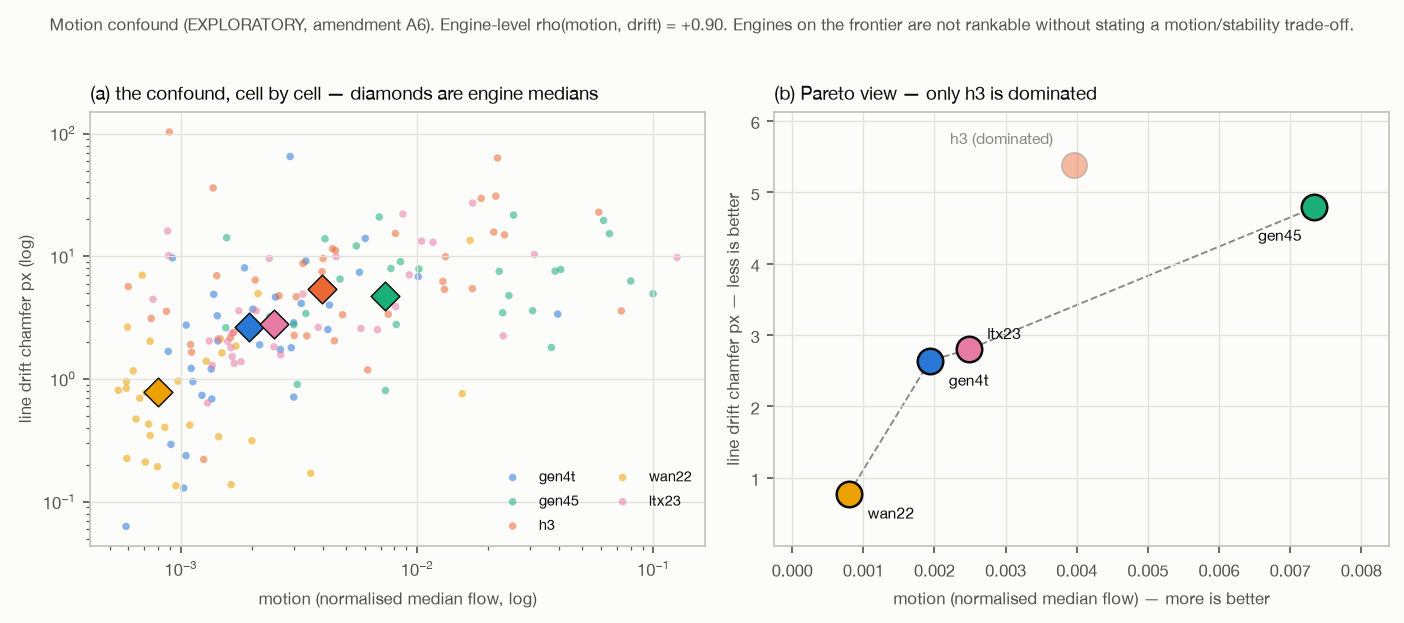
\includegraphics[width=\linewidth]{../analysis/out/figures/fig6_motion.png}
\caption{Motion confound (exploratory, amendment A6, motion, 2026-08-14). (a) Per-cell motion
against line drift, engine medians as diamonds: the association is visible
cell by cell and holds within four of five engines. (b) The engine-level
Pareto view: rightward is more motion, downward is less drift, so an engine
is dominated only if another lies right of and below it. Only H3 is dominated.
The dashed frontier is not a ranking. Engine codes in the figure: gen4t =
Gen-4 Turbo, gen45 = Gen-4.5, h3 = MiniMax H3, wan22 = Wan~2.2, ltx23 =
LTX-2.3.}
\label{fig:motion}
\end{figure}

Motion ordering is class-consistent on the calm end (IDLE is the calmest
class for Turbo, Gen-4.5 and LTX), but the peak differs (BURST breaks
Turbo; the CAMPUSH push-in breaks Gen-4.5 and LTX). H3 inverts the ordering
entirely: its mean line drift under IDLE (15.7\,px) exceeds its CAMPUSH mean
(6.2\,px). Its pathologies (ground inversion, hallucinated lettering, a
terminal blackout) are prompt-independent.

\subsection{The pre-registered hypothesis test: null, ten of ten}

The registered hypothesis, from the pilot study, was that
establishing-environment panels degrade more than character and action
panels on the edge and style headlines. The registered test (one-sided
exact Mann--Whitney U, establishing vs pooled others, per engine,
$\alpha=0.05$, rank-biserial effect sizes) is null on all ten
engine--metric combinations, on both the primary 33-cell basis and the
frozen-27 sensitivity basis (minimum $p=0.137$, LTX edge). Only LTX (edge,
$r=+0.24$) and H3 (style, $r=+0.20$) trend appreciably in the hypothesised
direction (LTX style $r=+0.13$ and H3 edge $r=+0.03$ are also positive but
smaller);
Turbo trends opposite on style ($r=-0.28$); its establishing panels were
its most stable. As registered, we state the small-$n$ caveat (12 vs 21
cells per engine; Turbo 12 vs 20): this is a non-replication under a
low-power test, not evidence of absence. Two notes of
context: the pilot plate that generated the hypothesis was refused
dataset clearance and is absent, and the establishing probes that are
present are the most line-stable class by mean chamfer on every engine while
carrying the matrix's largest edge outliers on four. The hypothesis may
yet hold for wash-heavy establishing plates, a dataset-composition question
we flag for extension rather than a settled negative.

\subsection{Treatment structure and the grey-ground covariate}

Ink treatment predicts failure better than content class. The heavy-blacks
column is H3's disaster zone (mean edge $|$slope$|$ 2.05 vs 0.17 on
line-only): dark grounds invite wholesale reinterpretation. The
chain-provenance cosmic panel is the hardest single panel for LTX and
Gen-4.5 (each engine's matrix-wide edge maximum) while Wan holds it almost
perfectly---except for inserting a cyclist into it
(Section~\ref{sec:taxonomy}). The creator-IP action panel is
engine-dependent: its treatment column is H3's cleanest, it is LTX's single most stable
cell, yet among Turbo's least stable on chamfer and style.

An exploratory observation (labelled as such; not pre-registered): the source-panel
paper-white p90 covariate correlates negatively with terminal style drift
on line-only cells for \emph{all five engines} (Spearman $\rho$ from $-0.10$
to $-0.83$). A grey ground is ambiguous about what the panel \emph{is}, and
each engine resolves the ambiguity in its own direction: one empties it
to white, one re-papers or inverts it, one flips figure and ground.

\subsection{First-to-last conditioning}

All six FLINT cells completed, and the headline observation is
architectural: first$\to$last conditioning can transport between two panels
\emph{without leaving the drawn register}: the interpolation lands on the
target panel in clean line-only ink after a transient mid-clip spot-black
flash. Register and content are separately controllable. (FLINT
vs-frame-0 scalars measure the intended transport plus drift and are
excluded from every cross-engine comparison, including the motion analysis
of Section~\ref{sec:league}; the released tables report them in a separate
column.)

\subsection{Repeat stability: failure modes are hazards, not properties}
\label{sec:repeat}

An authorised extension repeated the full 33-cell matrix on all three hosted
engines. \textbf{Engine-level conclusions are reproducible and per-cell
scores are not.} Every one of the five headline orderings is identical
across runs (Spearman $+1.00$), while per-cell agreement between runs ranges
from $+0.78$ down to $+0.08$ by engine and metric. MiniMax H3, the engine
with the most diverse pathologies, is also the least reproducible
(closure $+0.08$, i.e.\ no correlation).

One accident makes the point exactly. The ground series of
Section~\ref{sec:ground} includes an identity variant ($k=1.00$), which is
pixel-identical to its source panel (verified: maximum absolute difference
zero). Three independent draws of the same (panel, prompt, engine) triple
therefore exist, and their mean chamfer values are \textbf{103.1, 1.45 and
51.7\,px}---the corpus maximum and a near-perfect clip from identical
inputs.

This accident supplies something a benchmark normally has to design for: an
empirical noise floor. Yan et al.~\cite{yan2020cleanup} calibrate cleanup
algorithms by asking not only how far an output sits from a ground truth but
how far the multiple valid human ground truths sit from \emph{each other},
and treat the latter as the target an algorithm should reach. The generative
analogue is the spread between draws of one input, and here that spread
covers essentially the entire range of the metric. Any single-draw chamfer
value for this engine must be read against a floor of that width.

Review of the repeat clips shows the same structure qualitatively. The framing escape of
Section~\ref{sec:taxonomy} did not recur; the woodcut transposition
re-resolved as a volumetric light shaft (partial collapse); a terminal
blackout came back as a clean push-in to ground level that left the players almost entirely out of frame (a C1-style framing escape); and the pseudo-text violinist returned
as clean line-only ink with no lettering at all. What \emph{did} recur was
structured: the two heavy-black BURST cells departed hard in both draws,
one cutting to a lettered title card and then to a fish graphic, the other
to a speedline burst and then to a character on a brush-wave. Risk is
conditioned on motion class $\times$ ink treatment, and hallucinated
lettering is one possible landing of a broader graphic-cut hazard rather
than a property of those panels. Separately, the hallucinated train
reproduced but only transiently the second time, passing through frame and
exiting, which the terminal style scalar missed entirely (0.578 vs 0.062):
terminal-frame scalars under-report transient events where series maxima do
not.

Three consequences for benchmark practice. Single-draw scores are samples
from a per-input hazard distribution and should be reported as such;
engine-level rankings nonetheless survive replication and are the safe unit
of claim; and a named failure mode describes an outcome that a draw may
produce, not a property of the input that produces it.

\paragraph{Relation to depth-oriented evaluation in language models, and an
apparent disagreement.} The second of those consequences appears to
contradict the LLM safety literature that motivates this analysis. Broadwater
reports that models with comparable shallow-evaluation scores exhibit
substantially different failure rates under repeated sampling, and lists
cross-model rank divergence between $N=1$ and $N \gg 1$ among the effects
that depth
exposes~\cite{broadwater2026apst,broadwater2026reliability};
we find rankings that replicate exactly. The two results are consistent, and
the reconciliation is the level of aggregation. Our per-cell agreement is
weak (as low as $+0.08$), which is the same instability that work
describes. A headline ordering, however, is a median over 33 cells, and the
between-engine differences we rank are large relative to the residual draw
noise after that averaging; prompt-level comparison at $n \leq 3$ has neither
advantage. The practical statement is not that visual generation is more
stable than language generation, but that stochasticity binds at the unit of
report: our engine league is safe at $n=2$, our per-cell scores are not, and a
benchmark should say which of the two it is making claims about. Independent
support for the aggregate half comes from an unrelated direction: work on
deanonymising text-to-image leaderboards finds that repeated generations from
one model cluster tightly enough in embedding space, relative to the
separation between models, to identify the model that produced
them~\cite{naseh2026identifying}: between-model structure surviving
within-model draw noise, measured for a different purpose.

We note the corresponding limit on our own design. Establishing that a
failure mode \emph{occurs} as a draw needs few repeats; estimating its
\emph{rate} needs many more, and in the reference work failure probabilities
stabilise only after roughly 20--50 samples per
prompt~\cite{broadwater2026reliability}. At $n=2$ we report
existence and structure, not rates.

\subsection{Ground value is causal where draw noise permits the claim}
\label{sec:ground}

A second authorised extension (amendment A3) converted the exploratory
grey-ground covariate into a designed manipulation: five derived variants of
one line-only panel, pixel-identical up to a global luminance scale
($k \in \{1.0, 0.9, 0.8, 0.65, 0.52\}$; measured p90 1.000--0.518), each
run under IDLE. On Gen-4 Turbo the response is a threshold: stable to
p90${\approx}$0.8 (2.7--4.7\,px), then line drift climbs to 7.8 and
15.8\,px: $3.4\times$ from true white to the greyest ground and
$5.1\times$ from the last stable step (3.1\,px). The edge channel spikes only at the greyest
step and is non-monotonic across the middle steps, so this result rests on
the chamfer channel. (A3 named the monotonicity of terminal style drift and
edge $|$slope$|$ as its read-out; on Turbo neither is monotone, with five-point
$\rho$ against $k$ of $-0.5$ and $-0.4$, so the threshold is read from a
registered scalar, not from the registered read-out.) On Gen-4.5 the response is
flat-to-inverted: terminal style drift is \emph{highest on true white}.
On H3 the series is not interpretable at all: its $k=1.00$ point is one of
the pathological draws documented above, not a ground effect. Of the two
open-weights engines, LTX-2.3 drifts most on the greyest grounds (chamfer
10.0, 1.5, 13.4, 19.8 and 27.1\,px from true white to the greyest step) and
Wan~2.2 inverts (1.9, 1.3, 1.4, 0.1 and 0.1\,px: greyer grounds drift
\emph{less}).

That last observation yields a rule we now state with the experiment: an
$n=1$ dose series is readable only where per-draw variance is small relative
to the dose effect, and a repeat probe is what supplies the yardstick. Here
Turbo's between-run median $|\Delta|$ of 0.87\,px sits far below its
4.7--15.8\,px effect (readable); Gen-4.5's 1.54\,px against 5.8--12.3\,px is
marginal; H3's 102\,px maximum swing dwarfs anything the manipulation does.
The exploratory correlation (Turbo $\rho=-0.83$ vs Gen-4.5 $-0.29$) is thus
established as causal where it was strong, and left unestablished where it
was weak: ground value is an ambiguity that some engines resolve
destabilisingly and others do not, rather than a universal destabiliser.

\paragraph{The obvious alternative explanation, tested and rejected.} A grey
ground might destabilise nothing and merely provoke \emph{more motion}, with
the frozen metrics scoring that motion as drift, the same confound that
undermines the engine league in Section~\ref{sec:league}. The exploratory motion
channel lets us check. On Turbo, motion does fall as the ground darkens
($\rho(k, \text{motion}) = +0.70$), so motion co-varies with the ground and the
concern is live rather than hypothetical, if in the opposite direction; but the ground--drift relationship \emph{strengthens} once motion
is conditioned out, from $\rho = -0.70$ to $-0.80$. LTX behaves the same way
($-0.90 \rightarrow -0.98$), Wan's inverted response survives
($+0.80 \rightarrow +0.76$) and Gen-4.5 stays flat ($+0.30 \rightarrow 0.00$).
The ground effect is therefore not a motion artefact on the engines where it
was called causal. These are five-point rank coefficients on a five-step
series and we report them as descriptive support for a claim established by
the dose series itself, not as an independent test.

\subsection{Refusal asymmetry}

Identical inputs met three compliance behaviours: Gen-4 Turbo refused one
tone panel deterministically (twice, zero credits, an opaque server error);
Gen-4.5 output-moderated a different cell once and
passed it on the identical registered resubmission (a stochastic,
version-dependent safety layer); H3 generated everything, including both
cells above. The repeat probe extends this: the Turbo refusal reproduced
identically in the repeat run (four identical rejections across two days,
the only deterministic behaviour the probe found anywhere), while a second
Turbo cell failed then passed on identical resubmission and the Gen-4.5
moderation did not recur. Compliance boundaries are themselves stochastic at the margin
and version-dependent, which benchmark protocols must record.

\section{Failure taxonomy}
\label{sec:taxonomy}

The seeding rule was frozen before the study: a mode is named only with
$\geq 2$ independent exemplars (different panels or engines), and every
named mode states the metric signature that detects it, or that none
does. Seven modes met the rule, on three axes; severity on the register axis
is a ladder (drawn-but-more $\to$ drawn-but-different $\to$ not-drawn).

\paragraph{How the exemplars were established, and by whom.}
Candidate cells were first identified by mining metric outliers across the
corpus. Each candidate was then reviewed as a frame strip (source panel plus
three frames per clip) in six independent passes, and those passes were
performed by separate instances of an AI assistant, each shown only the
strips and asked to describe what changed (ground, line, tone, subject,
added content) without being told the candidate mode names or the
hypotheses under test. The author subsequently verified the resulting
exemplar descriptions against the same strips. We state this explicitly
because it is a limitation as well as a method: the qualitative observations
underpinning the taxonomy are AI-assisted and human-verified rather than
independently human-coded, and inter-coder reliability among human coders was
not measured. Every strip is released with the benchmark, so each exemplar
claim in this section can be checked directly by a reader. The quantitative
signatures attached to each mode are computed by the released metric code and
do not depend on the review passes.

\textbf{A. Register axis.}
\emph{A1 Register enrichment.} The engine stays ``ink'' but adds ink
vocabulary the source never had (screentone on skin, hatching, spot blacks);
detectable: tone variance fires on line-only panels.
\emph{A2 Register transposition.} Wholesale re-rendering into a different
ink idiom (noir wash re-cut as woodcut; line-on-grey flipped to inverted
scratchboard; silhouettes replaced by a speedline impact burst, the
matrix's largest edge slope at $+8.28$). Still monochrome ink to a human
eye; the metrics read catastrophe. A dated note in the released taxonomy records that A2 as seeded spans two behaviours (restyling the same scene, and abruptly replacing it with a different picture, the speedline burst) and proposes a split, not applied here, under which each half would still clear the seeding rule.
\emph{A3 Register collapse.} Departure towards photographic or painterly
rendering; catastrophic in pre-benchmark pilots, partial in-matrix
(volumetric searchlight glow; a face smoothed into gradient modelling).
The signed edge slope separates its softening and texturising forms.
(\emph{Candidate, unnamed at $n=1$:} a transient mid-clip monochrome break,
in which for one mid-clip stretch the whole ground renders as salmon-pink halftone and then recovers.)

\textbf{B. Content axis.}
\emph{B1 Element insertion.} New in-register content: a cyclist riding
out of an empty ice field; an entire subway train arriving at an empty
platform; a gloved hand entering a close-up. Signature: \textbf{geometry-quiet}.
The cyclist's 0.47\,px chamfer sits at the corpus's tenth percentile (eighteenth-lowest of 170 cells), with
closure and tone below the corpus median, while terminal style shows only
an unremarkable 0.248 (the corpus's 69th percentile) that no outlier screen would flag. No global scalar sees
localised insertion for what it is; this is the strongest single
argument for human validation and for per-region metrics.
\emph{B2 Pseudo-text insertion.} Hallucinated lettering: cursive
gibberish written beside a violinist; a night market replaced by a
brush-lettered title card; glyphs around a hallucinated dial. The
comics-trained prior expects text on ink panels and supplies it. Signature:
a step-jump-to-plateau in the chamfer \emph{series}, a shape feature rather than
a headline scalar.
\emph{B3 Content evacuation.} The drawing leaves: two engines ended
camera-push cells on an edge-to-edge black frame; a burst cell emptied to
bare paper as the subject exited. Signature: the edge terminal ratio collapses towards zero (the two blackout cells are the corpus's two lowest, $0.0007$ and $0.008$); the closure proxy moves but does not vanish.

\textbf{C. Framing axis.}
\emph{C1 Framing escape.} The camera runs away: an extreme close-up
zoomed out to a full-body long shot (same character, entire body invented);
push-ins that swallowed their scene. Identity often survives; composition
does not. Signature: chamfer and style fire hard, so globally it is
indistinguishable from register failure (the second blindness direction). A
framing-escaped clip with a perfect register scores like a broken one.

\section{Human check}
\label{sec:human}

\paragraph{Protocol as registered, and as amended.} The frozen protocol:
twenty clips drawn from the manifest by a fixed, recorded seed under
stratification constraints (every engine $\geq 3$, every content class
$\geq 6$, every motion class $\geq 6$); the author plus recruited raters;
five-point Likert ratings with the source panel alongside, clip order
randomised per rater, engine identity hidden;
analysis by Spearman $\rho$ per metric headline against mean rating with
bootstrap confidence intervals (CIs), and Krippendorff's
$\alpha$ for reliability. The kit and analysis scripts, committed before any
rating, implement these as a fixed per-rater order seed, 10{,}000 seeded
bootstrap resamples and the ordinal $\alpha$. Three dated amendments, each recorded before any
recruited rating existed, changed the instrument and its delivery; the analysis
machinery (Spearman $\rho$ with bootstrap CIs, ordinal $\alpha$, fixed
seeds) was untouched, though the amendments extended where it applies: A6
(instrument) ran it separately per axis to match the two-question instrument, and A8
registered a conditional re-expression of the register axis (whose outcome is
reported below) and the author-exclusion sensitivity analysis.

\emph{A6} (instrument, 2026-08-15): the original single endpoint-anchored
question measured one axis while the metrics respond to three, so the
instrument became two questions per clip (every scale point labelled): \emph{register} (``Does this clip still look like a hand-drawn
black-and-white ink picture, all the way through?'') and \emph{sameness}
(``Apart from the movement itself, is this the same original image
throughout?''), with guidance distinguishing continuation of depicted action
from invention of new content; the author's subsequent full pilot pass on the
revised kit scored the register question 5 on all twenty clips (zero
variance), confirming the original single-question instrument would have
yielded an unanalysable study (the pilot file is quarantined and never
pooled; the author then re-rated all twenty clips on the revised instrument,
and that second pass is the one pooled). \emph{A7}: delivery moved from an offline kit
to a hosted instrument behind per-rater authentication, with the question
wording machine-verified identical to the kit the pilot rater used (the
register question's bottom label and guidance note were revised after that
pass, under A6 addendum~4 and A8, before any recruited rating), an
offline download retained as a submission fallback, and passively recorded
timing fields declared exploratory under a no-exclusion rule registered in
advance. \emph{A8}: a \emph{baseline} question (``Does this original still image look
like a hand-drawn black-and-white ink picture?''), asked once per distinct
source panel before any clip (14 panels serve the 20 clips), because the register question is an absolute judgement with no
anchor, and a low register score on a panel that never read as ink would
otherwise be charged to the engine. The $\alpha$ implementation was verified
against the reference \texttt{krippendorff} package (maximum discrepancy
$2.2\times10^{-16}$ across the study data and adversarial synthetic cases)
before any value was read.

\paragraph{Pool.} Six raters: the author (whose clip pass was completed and
locked before the pool opened) and five recruited raters, each of whom completed the
full instrument in one sitting; of the six recruited slots the protocol
provided, one remained unfilled at analysis, and its later addition is
permitted. No rating was
excluded; none may be (registered rule). Play-through and dwell telemetry
were recorded passively (amendment A7) as exploratory fields, are not analysed here,
and are withheld from the release.

\begin{table}[t]
\centering
\small
\begin{tabular}{lcccc}
\toprule
& \multicolumn{2}{c}{Register ($\alpha = 0.21$)}
& \multicolumn{2}{c}{Sameness ($\alpha = 0.48$)} \\
\cmidrule(lr){2-3}\cmidrule(lr){4-5}
Metric headline & $\rho$ & 95\% CI & $\rho$ & 95\% CI \\
\midrule
line drift (chamfer)   & $-0.24$ & $[-0.69,+0.30]$ & $-0.42$ & $[-0.77,+0.04]$ \\
tone variance$^{\dagger}$ & $-0.32$ & $[-0.72,+0.18]$ & $\mathbf{-0.54}$ & $[-0.85,-0.08]$ \\
edge $|$slope$|$       & $\mathbf{-0.60}$ & $[-0.80,-0.22]$ & $\mathbf{-0.74}$ & $[-0.89,-0.43]$ \\
style (terminal)       & $-0.43$ & $[-0.77,+0.03]$ & $\mathbf{-0.64}$ & $[-0.83,-0.31]$ \\
closure $|$terminal$|$ & $\mathbf{-0.46}$ & $[-0.79,+0.01]$ & $\mathbf{-0.57}$ & $[-0.82,-0.17]$ \\
\bottomrule
\end{tabular}
\caption{Spearman $\rho$ between each frozen metric headline and the mean
human rating per axis ($n = 20$ clips; $^{\dagger}n = 16$, the tone metric
being undefined on four cells). Bold: $p < 0.05$ (asymptotic). The closure--register
interval brushes zero at the bootstrap resolution while its asymptotic
$p = 0.044$; we flag rather than hide the discrepancy. All ten correlations
carry the expected negative sign (higher metric $=$ more degradation
$=$ lower rating).}
\label{tab:human}
\end{table}

\paragraph{Results: the anchored axis works.} Table~\ref{tab:human} reports
both axes. On \emph{sameness}, the axis that anchors itself because the original
is on screen, four of five metrics correlate significantly with human
judgement, led by edge $|$slope$|$ at $\rho = -0.74$
($p = 2\times10^{-4}$), and inter-rater reliability is $\alpha = 0.48$. On
\emph{register}, only edge ($-0.60$) and closure ($-0.46$) reach
significance and reliability is $\alpha = 0.21$. Edge $|$slope$|$ is the
suite's standout, significant on both axes. All ten correlations are
negative, the sign fixed in the released analysis script before any rating,
and all five metrics track sameness more strongly than register, the
direction amendment A6 registered before any rating.

\paragraph{The baseline explains the weak axis.} The five recruited raters
agree usably on the per-panel baseline (mean pairwise $\rho = 0.42$;
Spearman--Brown reliability of the five-rater mean $0.79$; ordinal
$\alpha = 0.19$, lower because $\alpha$ also penalises the between-rater
level differences reported below), and what they
agree on is that the corpus is contested: three of fourteen panels reliably
do \emph{not} read as hand-drawn (naive means $1.60$, $1.80$, $2.00$; the
first near-unanimous at standard deviation $0.49$), and those three panels serve six of the
twenty clips. Three panels read clearly as ink ($\geq 4.0$). The cleanest
demonstration is a clip whose metrics are near-perfect (chamfer
$0.19$\,px, style $0.011$) yet whose register rating is $2.8$: its source
panel's own baseline is $2.0$, so the clip inherited a deficit no engine
behaviour caused. A low register score on this corpus is partly a corpus
property, which is what the baseline was registered to detect.
It is also the opposite of what the amendment predicted (baselines high and
low-variance, most panels at 4--5): the branch it called the more
consequential outcome is the one that fired.
The amendment's registered remedy, however, \emph{fails on its own terms}:
re-expressing register as the within-rater difference (clip minus panel
baseline) lowers reliability further ($\alpha = 0.21 \to 0.09$) and weakens
the three strongest correlations (edge $-0.60 \to -0.28$, closure
$-0.46 \to -0.34$, style $-0.43 \to -0.26$), leaving none significant. This is the familiar unreliability of difference scores
composed of two noisy terms~\cite{cronbach1970change}. We therefore report
the register axis at level, with its baseline caveat, and do not attempt to
rescue it.

\paragraph{Per-mode predictions stated in advance.} Before any rating, we
recorded three expectations in the project's dated findings log (2026-08-12;
these are not part of the pre-registration). (i)~\emph{Insertion cells would divide
metrics from raters}: confirmed on the subset's B1 exemplar, where the
hallucinated cyclist scores chamfer $0.47$\,px, indistinguishable from the
subset's best cells, yet raters score its sameness $2.0$. The taxonomy's monochrome-break
candidate is the concordant contrast: a register-axis event, not an
insertion, on which metrics and raters agree: it tops the subset on style
($0.618$) and edge slope, and is its unanimous sameness floor ($1.0$,
standard deviation $0$). (ii)~\emph{Transposition cells would be rated
more ink-plausible than their metric scores imply}: not testable, because the
frozen subset, drawn by declared seed under the frozen stratification and
without reference to the taxonomy, contains no A2
cell, a coverage gap we report rather than repair. (iii)~\emph{Disagreement
would be highest on transposition}: not testable for the same reason.

\paragraph{The result does not hinge on the author.} The pre-registered
sensitivity analysis re-runs everything excluding the author: every
correlation keeps its sign, sameness $\alpha$ is stable ($0.48 \to 0.49$),
and register $\alpha$ \emph{improves} ($0.21 \to 0.32$). The author is
the register-axis outlier, not its warrant. The direction is consistent with
the baseline: the author's panel baselines average $4.64$ against the naive
pool's $3.19$, a $+1.46$ gap (computed before rounding); one recruited rater matches the author exactly
($4.64$), the severest sits at $2.07$. How ``hand-drawn'' a synthetic ink
panel looks is substantially rater-dependent, and the person who made the
corpus sees it most favourably. We report that as a finding about benchmark
construction, and let the recruited pool carry the corpus-facing judgement.

\section{Limitations}

Single-author study; every protocol element that protects against
solo-lab degrees of freedom (freeze, amendments, ledger, released nulls) is
in the repository, but replication is the real control. The registered test
is low-power by design (33 cells per engine; the null is a non-replication,
not a demonstrated absence). Global scalars conflate composition change
with register change in both directions (A2/C1 vs B1); per-region
metrics are the natural extension. One engine's cells run at its native
$1344\times768$ grid vs $1280\times720$/$1280\times704$ elsewhere; chamfer
is defined at native resolution as frozen, and a per-diagonal sensitivity
column changes no ordering. Model churn is pinned per clip (version strings,
dates; execution hardware per batch, Table~\ref{tab:engines}) but hosted engines are moving targets: one moderation
outcome in this study was already nondeterministic across identical
submissions. Execution disclosures: 22 hosted cells were accidentally
submitted twice by concurrent drivers (billed, reconciled; the operative
generation is fixed by a rule set before scoring); one cell's style metric
was re-scored after a transient weight-download failure (audited, byte-level
scope); one FLINT cell's edge headline is undefined (zero frame-0 gradient).
Single seed per cell; seed-variance, open-weights-vs-API, and tone-density
ablations are named, budgeted extensions.

\textbf{The motion confound is real, measured, and only partly
mitigated.} Every metric in our suite is optimised by a clip that does not
move. This is a known hazard in video-generation evaluation rather than a
peculiarity of ours. VBench observes that ``generating relatively static
scenes can `cheat' to get high temporal consistency scores'' and pairs its
consistency dimensions with a Dynamic Degree control estimated from optical
flow~\cite{huang2023vbench}. Section~\ref{sec:league} quantifies the damage
for our corpus: engine-level motion and line drift rank together at
$\rho = +0.90$, and the five engines' motion ranges have no common overlap,
so no matched-motion comparison of all five is available. The remedy we apply, reporting the
league beside its motion medians and declining to call it a quality ranking,
is a disclosure, not a fix. A benchmark that wanted a clean quality ordering
on this substrate would need motion held constant by construction, for
instance by scoring only cells whose realised motion falls in a common band,
which our corpus cannot supply. The motion channel itself is post-hoc and
exploratory (amendment A6, motion, 2026-08-14); it is not one of the five frozen metrics, is not
used to restate any frozen result, and its definitions were fixed only after
the corpus was complete.

\textbf{Tone metric at the extremes.} \texttt{tone\_spectral\_drift} measures
variance in screentone band energy, and a region of uniform intensity has no
screentone variation to measure. At the extremes of the ground series the
metric is therefore partly constrained by definition rather than by engine
behaviour, and the ground result should be read from the chamfer and edge
channels, as reported.

\textbf{Rater pool.} The human check uses six raters, small against
perceptual studies in the graphics literature: Yu et
al.~\cite{yu2024sketchbeaut} recruit 23 participants for a preference
vote. The comparison is not exact: that design contrasts competing methods
and needs power across participants, whereas ours correlates per-clip
ratings against metric values; for that case ImagenHub settles on three
raters per model, having found that Krippendorff's $\alpha$ \emph{falls} as
raters are added~\cite{ku2023imagenhub}, an effect our own data echoes in
one direction (register $\alpha$ rose when the author was excluded). Axes
and the reliability statistic were fixed before any rating, and the pool
composition before any recruited rating (amendments A6~(instrument), A7 and A8). Known
asymmetries of the pilot rater are on record and none is repairable
post-hoc: the author rated before the baseline task existed (so has no
baseline-first warm-up), under an offline kit rather than the hosted
instrument (question wording machine-verified identical; the register label
and guidance note were revised afterwards under A6 addendum~4 and A8), knows
the hypotheses,
and lacks per-clip timing telemetry. The register axis is additionally
bounded by the corpus itself (Section~\ref{sec:human}); its registered
difference-score remedy failed for the standard
reason~\cite{cronbach1970change} and is reported failed rather than
replaced by an unregistered alternative. Finally, our repeat
depth ($n=2$) establishes that failure modes occur as draws and how that risk
is structured, but is far short of the depth needed to estimate per-cell
hazard \emph{rates}~\cite{broadwater2026reliability}; the one ten-draw
measurement we made (amendment A4: eight cells on a single engine) is released
with its registered null and is not analysed here.

\section*{Data and code availability}
The release archive (DOI~\datadoi) contains the 29 benchmark panels with
their line-art layers, recipes, and datasheet; the five ground-series
variants; all 373 generated clips with the per-clip manifest and metric
outputs; the frame strips reviewed for the taxonomy; the frozen
pre-registration with its amendments; the budget ledger; the aggregated
human-check results with the rating instrument; and the metric, harness, and
analysis code (less the two thin engine-client wrappers the harness calls, as
\texttt{harness/README.md} explains). Data are released under CC~BY~4.0 and code under the MIT
licence; the code is also at \coderepo. Release copies differ from the
generation outputs only in metadata: embedded generator graphs were removed
from panel files, one panel identifier was neutralised, and absolute paths in
the manifest and metric files were made relative, with pixel and
video content unchanged and every change and file hash listed in the
archive. Human-check ratings are released as pseudonymised per-rater scores (opaque
codes for the five recruited raters, and the author's own file labelled by
name; no names or contact details were collected, and answer
timestamps, timings, and comments are withheld), so the reliability statistics
and correlations reported above can be recomputed. Items generated through commercial
services carry a provider-terms notice (\texttt{NOTICE-PROVIDERS.md}, referenced
from the datasheet).

\section*{AI-use disclosure}
The author used Claude (Anthropic) agentic tooling to assist with software
development for the generation harness, metric implementation, analysis and
figure pipeline; with the structured frame-strip review passes that
established the taxonomy exemplars (Section~\ref{sec:taxonomy}, where the
procedure and its limitations are described in full, and whose underlying
strips are released for independent checking); with preparing the data
release; with drafting the working records released alongside the paper
(pre-registration amendments, budget-ledger entries, taxonomy notes), which
were written under the author's direction and are released verbatim apart
from the redactions of private operational detail listed in the archive, partly
in the assistant's voice; and with drafting and editing this text. All
panels, clips,
and measurements derive from the benchmark runs described above; no research
data, measurements, or results were generated, synthesised, or altered by AI
beyond the disclosed use of generative image/video engines as the
\emph{objects of study}. The author reviewed and verified all analyses,
numerical results, figures, and text, and takes full responsibility for the
content.

\bibliographystyle{IEEEtran}
\bibliography{refs}

\end{document}

